\documentclass[a4paper]{book}

\usepackage{draftwatermark}
\SetWatermarkText{Draft}
\SetWatermarkColor[gray]{0.9}

\usepackage[utf8]{inputenc}
\usepackage[T1]{fontenc}

\usepackage{titlesec, blindtext, xcolor}
\definecolor{gray75}{gray}{0.75}
\definecolor{base00}{HTML}{fafafa}
\definecolor{base01}{HTML}{d4d4d4}
\definecolor{base02}{HTML}{abacae}
\definecolor{base03}{HTML}{7e8087}
\definecolor{base04}{HTML}{555761}
\definecolor{base05}{HTML}{333333}
\definecolor{base06}{HTML}{4d4d4d}
\definecolor{base07}{HTML}{666666}
\definecolor{base08}{HTML}{a10705}
\definecolor{base09}{HTML}{0d52bf}
\definecolor{base0A}{HTML}{cc3b02}
\definecolor{base0B}{HTML}{57392d}
\definecolor{base0C}{HTML}{d48e15}
\definecolor{base0D}{HTML}{3a9104}
\definecolor{base0E}{HTML}{7239b3}
\definecolor{base0F}{HTML}{667885}

\newcommand{\hsp}{\hspace{10pt}}
\titleformat{\chapter}[hang]{\Huge\bfseries}{\textcolor{base02}{\thechapter \hsp \vline}\hsp}{0pt}{\Huge\bfseries}
\titleformat{\section}[hang]{\Large\bfseries}{\textcolor{base01}{\thesection \hsp \vline}\hsp}{0pt}{\Large\bfseries}
\titleformat{\subsection}[hang]{\large\bfseries}{\textcolor{base01}{\thesubsection \hsp \vline}\hsp}{0pt}{\large\bfseries}

\usepackage[american]{babel}
\usepackage{csquotes}
\usepackage[style=apa,sortcites=true,sorting=nyt,backend=biber]{biblatex}
\DeclareLanguageMapping{american}{american-apa}
\addbibresource{references.bib}

% Essentials
\usepackage{tabularx}
\usepackage{graphicx}
\usepackage{subcaption}
\usepackage[ruled]{algorithm2e}

% Typography
\usepackage{palatino}
\usepackage{fontenc}

% Links
\usepackage[colorlinks=true, citecolor=base08, linkcolor=base08, urlcolor=base08]{hyperref}

% Math stuff
\usepackage{amsmath}
\usepackage{amssymb}
\usepackage{amstext}
\usepackage{bm}

% Commands
\DeclareMathOperator*{\argmin}{arg\,min}
\DeclareMathOperator*{\argmax}{arg\,max}

\begin{document}

\begin{titlepage}
    \begin{center}
        \huge\textbf{Composing like a human:} \\
        \Large\textbf{Adapting generative networks to few-shot learning in the musical domain}
        \normalsize

        \vspace{1cm}

        \textbf{Tudor Paisa}\\
        Student Number: 2019551 \\
        Administration Number: 315146\\
        t.paisa@tilburguniversity.edu\\

        \vspace{1cm}
        \textsc{Thesis submitted in partial fulfillment\\
        of the requirements for the degree of\\
        Master of Science in Data Science and Society,\\
        at the School of Humanities and Digital Sciences\\
        of Tilburg University\\}

        \vspace{2cm}
        Thesis Committee:\\
        Dr. Menno van Zaanen\\
        Dr. SECOND READER\\
        \vfill

        Tilburg University\\
        School of Humanities and Digital Sciences\\
        Department of Cognitive Science \& Artificial Intelligence\\
        Tilburg, The Netherlands\\
        \today
 
    \end{center}
\end{titlepage}

\chapter*{Abstract}
    Lorem Ipsum

\tableofcontents

\chapter{The return of the Neural Net}

Over the past sixty years, Artificial Neural Networks (ANNs) have experienced a number of cycles in popularity noted by extensive publicity of over-inflated expectations on the promises of connectionism (the field of science that tries to explain mental phenomena with the help of ANNs [CITATION NEEDED]): that a system could learn to do anything it was programmed to do [CITATION NEEDED] \parencite{minsky_perceptrons_1988}. However, each wave of praise was followed by a mass of public disappointment, criticism, and funding cuts [CITATION NEEDED]. These upturns and downturns of the field of connectionism - or more generally A.I. - are now known in the literature as the A.I. winters [CITATION NEEDED].

The recent revival of ANNs under the scope of Deep Learning (DL) has brought new ways to tackle Machine Learning problems, most notably in the context of classification (but also regression, although less popular; see \cite{lecun_deep_2015} for several examples of DL applications). In addition, with the advent of chatbots \parencite{dale_return_2016}, voice-activated personal assistants \parencite{xiong_microsoft_2018}, and general-purpose A.I. systems \parencite{vinyals_starcraft_2017}, DL introduced new frontiers in artificial intelligence research.

% NOTE: USE ME LATER
% Currently, two exciting areas of research in the field of Deep Learning (DL) are in designing generative models \parencite{goodfellow_nips_2016} and training NNs on small datasets \parencite{finn_model-agnostic_2017, nichol_first-order_2018}. This research will combine both of these tasks by exploring the extent to which generative models can create novel and qualitative samples of music under the constraints posed by the few-shot learning problem. In other words, when data is scarce, can a generative model create samples of music that are new (i.e., not in the training set), consistent with common scales, and diverse (tone sequences are not repeated over and over, combines chord structures with single-note sequences, is not restricted to - say - one octave). This research will evaluate the generated samples of two state-of-the-art generative models (C-RNN-GAN of \cite{mogren_c-rnn-gan_2016} and Performance-RNN of \cite{oore_this_2018}) that have been trained under the Reptile learning framework \parencite{nichol_first-order_2018} on small amounts of MIDI data.

Broadly speaking, DL as a field, promises to solve tasks which are easily (intuitively) performed by people, but hard to formalize \parencite[e.g., recognizing faces or spoken word;][]{goodfellow_deep_2016}. The solution comprises of enabling computers to learn form experience and understand the world through the discovery of hierarchical relationships between concepts \parencite{lecun_deep_2015}. This way, there is no need for manual input on the sort of knowledge that the computer needs \parencite{goodfellow_deep_2016}. A more simplistic and concise interpretation of DL would be to see it as a statistical technique for identifying patterns in sample data using large (deep) ANNs \parencite{marcus_deep_2018}.

The reasons for presenting these facts will be clarified in the following sections however, a terse argumentation is that progress towards general A.I. systems is marked by scant explorations of ANNs outside of the classification task, and even more so when trying to overcome some of their shortcomings, such as being highly reliant on massive amounts of data [CITATION NEEDED].
% NOTE: Maybe I was too harsh?

\section{We do not discriminate}\label{sec:no_disc}

Typically, in a neural network, the data samples go through a set of input units (that might represent pixels, word embeddings, etc.), then through multiple hidden layers, each with a given number of nodes, and reaching the output units where the answer is given \parencite{marcus_deep_2018}. An overwhelming majority of experiments with ANNs involve discriminative models \parencite{goodfellow_generative_2014}, where the goal is to assign the high-dimensional inputs to a class label \parencite[such as an animal or piece of furniture;][]{zhang_character-level_2015, krizhevsky_imagenet_2012}. However, other possible applications of DL models include (but are not limited to): regression [CITATION NEEDED], data compression \parencite{cheng_deep_2018}, and generating new data points \parencite{graves_generating_2013}.

For the purposes of this paper (see Section \ref{sec:thesis_goal}), generative model are central to our experiments (Chapter \ref{chap:methods}). Borrowing the analogy from \textcite{goodfellow_nips_2016}, one might wonder what is the value of studying generative models. After all, in the image domain, such a framework would merely generate more images (something which the Internet as no shortage of). Some of the more eloquent answers include using generative models for simulating possible futures to be later used for planning [CITATION NEEDED], providing predictions to missing data, or enabling work on multi-modal outputs, where a single input may have more than one correct answer \parencite{goodfellow_nips_2016}.

However, successes in generative models have been scarce, with Fully Visible Belief Networks \parencite{frey_does_1996} being the most suitable (and popular) method for the longest run. Yet, this method requires generating each sample one at a time (ramping up the cost of the process to $O(n)$). Coupled with the fact that the computation is done through a neural network, creating $n$ samples requires a substantial amount of time \parencite{goodfellow_nips_2016}. Variational Autoencoders \parencite{kingma_auto-encoding_2013} are another popular method that is used for this sort of task. Their main drawback is that when a weak approximation of a prior or posterior distribution of the data is used, the model might learn something other than the true data distribution \parencite{goodfellow_nips_2016}.

The discovery of Generative Adversarial Networks \parencite[GANs;][]{goodfellow_generative_2014} has leapfrogged the state of developments in this field. Besides countering the drawbacks outlined above \parencite{goodfellow_nips_2016}, they have been particularly successful at a variety of tasks such as image super-resolution \parencite[; see Figure \ref{fig:srgan}]{ledig_photo-realistic_2016}, style-based image generation \parencite{karras_style-based_2018}, or image-to-image translation \parencite[such as converting a satellite image into a map, or a sketch into a photorealistic image;][;see Figure \ref{fig:pix2pix}]{isola_image--image_2016}.

Although not as popular as the abovementioned, Recurrent Neural Networks (RNNs) have been successfully implemented for various generative tasks \parencite{jenal_rnn-based_2019, ICML2011Sutskever_524}. More specifically, a variation of these, Long Short-Term Memory Networks \parencite[LSTMs;][]{hochreiter_long_1997}, are of particular interest to this task. RNNs (and by extension LSTMs) contain a high-dimensional hidden state which allows them to remember and predict from previous inputs \parencite{ICML2011Sutskever_524}. This makes them great candidates for predicting sequences \parencite{graves_generating_2013} of text or characters, where the input at $t_0$ might be influenced by prior input at $t_{-1}$, $t_{-2}$, etc \parencite{fan_tts_2014}.

\begin{figure}[t]
    \centering
    \begin{subfigure}{.24\linewidth}
        
\includegraphics[width=\linewidth]{images/comic_HR.jpg}
        \caption{original}
        \label{fig:srgan_orig}
    \end{subfigure}
    \begin{subfigure}{.24\linewidth}
        
\includegraphics[width=\linewidth]{images/comic_SRF_4_bicubic.jpg}
        \caption{bicubic}
        \label{fig:srgan_bicubic}
    \end{subfigure}
    \begin{subfigure}{.24\linewidth}
        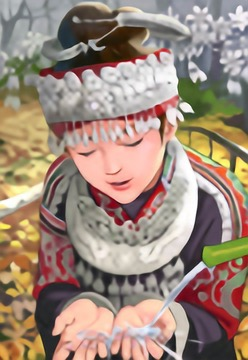
\includegraphics[width=\linewidth]{images/comic_SRResNet-MSE.jpg}
        \caption{SRResNet}
        \label{fig:srgan_srresnet}
    \end{subfigure}
    \begin{subfigure}{.24\linewidth}
        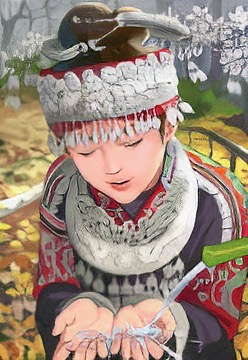
\includegraphics[width=\linewidth]{images/comic_SRGAN-VGG54.jpg}
        \caption{SRGAN}
        \label{fig:srgan_srgan}
    \end{subfigure}

    \caption{Example of single-image super-resolution results that highlight the advantages of a GAN. The original high-resolution image (\ref{fig:srgan_orig}) has been downsampled to make a low-resolution image. The results of bicubic interpolation (\ref{fig:srgan_bicubic}) can be seen in the second image, followed by the results of SRResNet (\ref{fig:srgan_srresnet}), a neural network trained on mean squared error. Lastly, the results of SRGAN can be seen in the final image (\ref{fig:srgan_srgan}). Figure adapted from \textcite{ledig_photo-realistic_2016}.}
    \label{fig:srgan}
\end{figure}

\begin{figure}[t]
    \centering
    \begin{tabular}{ccc}
    Input & Ground Truth & Output \\
    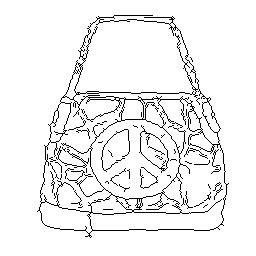
\includegraphics[width=.15\linewidth]{images/handbags_edges_lotsofresults_latex/input_106_AB.jpg} &
    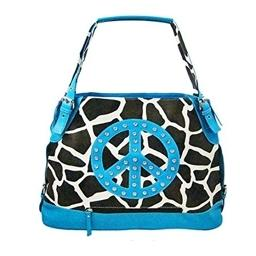
\includegraphics[width=.15\linewidth]{images/handbags_edges_lotsofresults_latex/gt_106_AB.jpg} &
    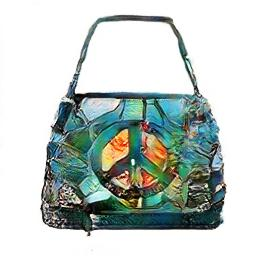
\includegraphics[width=.15\linewidth]{images/handbags_edges_lotsofresults_latex/L1cGAN_106_AB.jpg} \\
    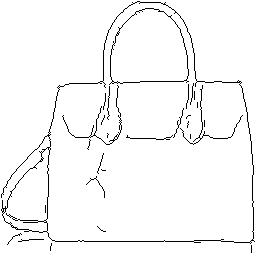
\includegraphics[width=.15\linewidth]{images/handbags_edges_lotsofresults_latex/input_12_AB.jpg} &
    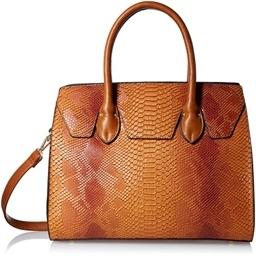
\includegraphics[width=.15\linewidth]{images/handbags_edges_lotsofresults_latex/gt_12_AB.jpg} &
    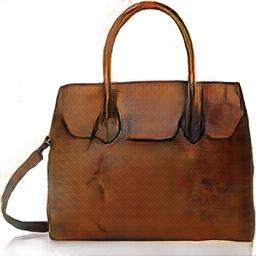
\includegraphics[width=.15\linewidth]{images/handbags_edges_lotsofresults_latex/L1cGAN_12_AB.jpg} \\
    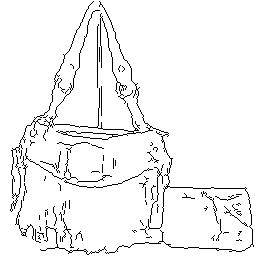
\includegraphics[width=.15\linewidth]{images/handbags_edges_lotsofresults_latex/input_130_AB.jpg} &
    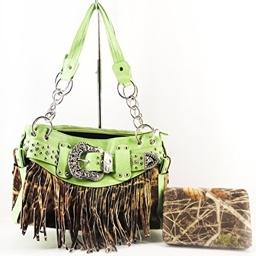
\includegraphics[width=.15\linewidth]{images/handbags_edges_lotsofresults_latex/gt_130_AB.jpg} &
    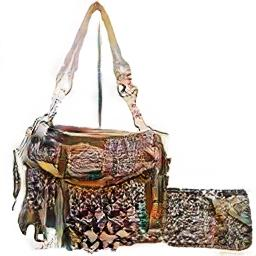
\includegraphics[width=.15\linewidth]{images/handbags_edges_lotsofresults_latex/L1cGAN_130_AB.jpg} \\
    \end{tabular}
    \caption{\textcite{isola_image--image_2016} coined the term image-to-image translation where an input image is transformed into a revisualization of the original input. This figures illustrates how an outline of a purse (leftmost column) is transformed into a colored photorealistic version of it (rightmost column). In the middle we have the ground truth: the real image of the purse. Figure adapted from \textcite{isola_image--image_2016}.}
    \label{fig:pix2pix}
\end{figure}

These developments in generative models lie in the field of Computer Vision, but that is not to say that we can generate only images. GANs (and others) have been applied - with varying degrees of success - in Natural Language Processing where the scope was to generate high-quality text with sufficient diversity \parencite[e.g.,][]{yu_seqgan_2016, chen_adversarial_2018}. Less explored, but still successful, have been the efforts in generating music \parencite[e.g.,][]{mogren_c-rnn-gan_2016, dong_musegan_2017}. This paper will focus on the problem of generating music with a NN-based model. Respectively, this paper will evaluate the samples generated by C-RNN-GAN \parencite{mogren_c-rnn-gan_2016} and Performance-RNN \parencite{oore_this_2018} when trained under the few-shot learning problem (detailed below).

\section{"Just... One more bite"}\label{sec:hungry}

It is fairly well known that DL models tend to be very "data-hungry", a caveat imposed by its optimization algorithm \parencite{chen_closer_2018, ravi_optimization_2016}. DL usually relies on a procedure called stochastic gradient descent (SGC) which implies computing for a given input vector the output and error, followed by calculating the input's average gradient and consequently adjusting the network's weights \parencite{lecun_deep_2015}. \textcite{ravi_optimization_2016} argue that the iterative nature of gradient-optimization algorithms does not allow them to perform well under the constraint of a set number of updates: when faced with non-convex optimization problems, DL algorithms do not guarantee convergence within a reasonable amount of time. Finally, they add by saying that for each new problem (e.g., new dataset), the model needs to reinitialize with a new set of random parameters which hurts the network's ability to converge to a good solution when constrained by a limited number of updates \parencite{ravi_optimization_2016}.

Besides the promise of making DL algorithms easier to train, primary reasons why this issue needs to be addressed are as follows. Firstly, humans have the ability to generalize after one (or few) example(s) of a given object \parencite{vinyals_matching_2016, chen_closer_2018, ravi_optimization_2016}, something which DL algorithms do not. Secondly, this would alleviate the constant need for data collection in order to provide reasonable performances. Finally, there are many fields where the data exhibits a large number of classes, with few examples per class and Bridging the gap between human-type learning and current learning architectures would allow models to properly capture this sort of data \parencite{ravi_optimization_2016, larochelle_few-shot_2017}. This is known as the few-shot problem \parencite{chen_closer_2018, vinyals_matching_2016, larochelle_few-shot_2017}.

\section{Making music like a hooman} \label{sec:thesis_goal}

In spite of its proposed benefits, developments and experiments in few-shot learning are still scarce \parencite{larochelle_few-shot_2017} and evaluations are largely concentrated on image data \parencite[see][]{lake_omniglot_2019, clouatre_figr_2019, vinyals_matching_2016, chen_closer_2018, ravi_optimization_2016}. Few-shot experiments with generative networks are even less frequent \parencite{zhang_metagan_2018, clouatre_figr_2019}. This research aims to explore the viability of this learning approach in the context of generating music data. More concretely, in light of recent developments, this research will evaluate two generative networks modelled on MIDI data under the constraints of few-shot learning, and comparing its performance to the baseline proposed by \textcite{larochelle_few-shot_2017} and properties extracted from real music performances.

\chapter{Related Work}

\textcite{lake_human-level_2015} initially popularized the idea of learning from a few class examples using a probabilistic learning framework capable of generalizing and learning a large number of concepts from a single class example (i.e., one-shot learning). \textcite{rezende_one-shot_2016} were among the first to provide a solution to the one-shot problem in the context of a neural network (NN) by implementing Bayesian reasoning into a deep NN embedded within hierarchical latent variable models. The Reptile algorithm \parencite{nichol_first-order_2018} is a recent approach to this problem. It counteracts the shortcomings of gradient-optimization algorithms by learning the model's initial parameters in order to maximize its performance on novel tasks. Furthermore, it allows for any type of network to be used and does not place any restrictions on the type of loss function that can be used \parencite{nichol_first-order_2018}. The algorithm for Reptile is as follows:

\IncMargin{1em}
\begin{algorithm}
Initialize $\phi$, the vector of initial parameters

\For{iteration = $1, 2, \dots$}{
    Sample task $\tau$, corresponding to loss $L_{\tau}$ on weight vectors $\tilde \phi$

    Compute $\tilde \phi = U_{\tau}^{k} (\phi)$, denoting $k$ steps of SGD or Adam

    Update $\phi \leftarrow \phi + \epsilon (\tilde{\phi} - \phi)$
}

\caption{Reptile (serial version)}
\label{alg:reptile}
\end{algorithm}
\DecMargin{1em}

Although simplistic, this algorithm reaches similar results to another popular few-shot algorithm called MAML \parencite{finn_model-agnostic_2017}. Both algorithms are initialization-based learning methods however, a major distinction between the two is that the vanilla MAML implementation requires calculating a second-order derivative, which can significantly slowdown computation \parencite{nichol_first-order_2018}. This forms a compelling reason to use Reptile as the few-shot learning method for this research.

Turning over to the generative side of things, nowadays, the most popular form of generating data is through the use of a Generative Adversarial Network \parencite[GAN;][]{goodfellow_generative_2014}. Here a generative model $G$ captures the data distribution and creates samples from it, whereas a discriminative model $D$ estimates the probability that the input is real (i.e., comes from the training data) rather than fake (i.e., comes from $G$). Formally, given $x$ sampled from real data, and $z$ being input noise, $D$ tries to keep $D(x)$ near $1$, while making $D(G(z))$ near $0$. Conversely, $G$ tries to make $D(G(z))$ near $1$ \parencite{goodfellow_nips_2016}. A notable implementation is C-RNN-GAN \parencite{mogren_c-rnn-gan_2016}, a continuous recurrent neural network with adversarial training. It consists of a network with two LSTM layers and 350 hidden units per layer, in both $G$ and $D$. However, $D$ has a bidirectional layout which allows is to take context from both past and future for its decisions, while $G$ is unidirectional \parencite{mogren_c-rnn-gan_2016}. As is the standard practice for GANs, $G$ will create fake samples of music, whereas $D$ will try to classify correctly which sample is real.

Notwithstanding GANs, other generative successes have made use of adaptation on the Long Short-Term Memory (LSTM) network \parencite{hochreiter_long_1997}. Here, the cells of a network are designed to allow for information to persist by implementing a recursive state unit, an input gate, a forget gate, and an output gate. The input of the network is allowed into the state unit if it is allowed to pass through by the input gate. Next, the forget gate controls the self-loop of the state cell. Finally, the output gate has the power to shut off the output cell \parencite{goodfellow_deep_2016}. Here, a notable implementation is Performance-RNN \parencite{oore_this_2018}; a three layer LSTM network with 512 layers each. Compared to C-RNN-GAN, here the network is completely unidirectional. Probably more important than the network architecture, a central piece of the model's performance is due to the final representation of the MIDI data: each time slice is represented as a one-hot encoded vector containing Note-On (128 values), Note-Off (128 values), Time-Shift (125 values), and Velocity (32 values) events \parencite{oore_this_2018}. 

C-RNN-GAN and Performance-RNN have not been tested and adapted to the few-shot learning problem, but more general GANs and LSTM networks have been \parencite[see][]{zhang_metagan_2018, vinyals_matching_2016}. However, as mentioned previously, no evaluation has been made in the musical domain. Therefore, this study will seek to answer the following research questions:

\begin{itemize}
    \item To what extent is the music created by a few-shot generative model comparable to the music of a generative model that is trained on the entire dataset?
    \item To what extent is the music created by a few-shot generative model comparable to real music?

\end{itemize}

\chapter{Methods}\label{chap:methods}

To provide an answer to the above research questions, this study will develop (in Keras) two generative models based on C-RNN-GAN and Performance-RNN, where the learning procedure will incorporate the Reptile algorithm. Other than that, the models will not differ from their original implementation. These models will firstly be compared to the baseline proposed by \textcite{larochelle_few-shot_2017} (a LSTM network trained on the entire train set) and then with the music from the dataset. The evaluation between the models with the baseline will be based on the number of statistically different bins \parencite[NDB;][]{richardson_gans_2018} and domain specific measurements (polyphony, scale consistency, repetitions, tone span). The evaluation between the model's generated samples and real music in the dataset will be based on the domain specific metric. Refer to the evaluation section for more details on these metrics.

\section{Dataset}

The dataset for this research will be similar to that of \parencite{oore_this_2018} namely, the MAESTRO Dataset \parencite{hawthorne_enabling_2018}. It consists of recorded MIDI data collected from each installment of the International Piano-e-Competition. All performances were done by piano experts on a Yamaha Disklavier, instrument which integrates a highly precise MIDI capture and playback system. Recorded MIDI events are of sufficient fidelity to allow judges to remotely listen to the contestant's performance (also on a Disklavier).

The dataset contains MIDI recordings from nine years of the International Piano-e-Competition. This amounts to 1,184 piano performances, approximately 430 compositions, 6.18 million notes played, and approximately 172 hours of playback. There is also a recommended train/validation/test split created on the following criteria \parencite{hawthorne_enabling_2018}:

\begin{itemize}
    \item No composition should appear in more than one split
    \item Training set is approx 80\% of the dataset (in time), and the remaining is split equally on between the validation and test sets. Where possible, these proportions are true also within each composer.
    \item Popular compositions are in the training set
    \item The validation and test splits should maintain a variety of compositions
\end{itemize}

Moreover, each performance comes with additional metadata namely, the name of the composer, the title of the performance, the suggested train, validation, test splits, year of the performance, name of the file, and duration in seconds of the performance.

\section{Evaluation}

Generally, DL models work by the principle of likelihood maximization, which simply says to choose the parameters that maximize the probability that the model assigns to the training data \parencite{goodfellow_nips_2016}. Formally, this means selecting the parameters that maximize $\prod_{i=1}^N p_{\text{model}}(\bm{x}^{(i)}; \bm{\theta})$:

\begin{equation}
    \bm{\theta^*} = \arg \max \prod_{i=1}^N p_{\text{model}}(\bm{x}^{(i)}; \bm{\theta}) \label{eq:og_mle}.
\end{equation}

However, calculating the product over many probabilities is prone to numerical problems such as underflow \parencite{goodfellow_nips_2016}. This is alleviated by calculating $\bm{\theta^*}$ in $\log$ space where the product is transformed into a sum:

\begin{equation}
    \bm{\theta^*} = \arg \max \sum_{i=1}^N \log p_{\text{model}}(\bm{x}^{(i)}; \bm{\theta}) \label{eg:log_mle}.
\end{equation}

That being said, calculating maximum likelihood can be thought of minimizing the Kullback-Leibler (KL) divergence: minimizing the dissimilarity between the data generating distribution $p_{\text{data}}$ and the model $p_{\text{model}}$. Thus, $\bm{\theta^*} = \argmin_{\bm{\theta}} D_{KL}(p_{\text{data}}(\bm{x}) \| p_{\text{model}} (\bm{x}; \bm{\theta}))$. The KL divergence is given by:

\begin{equation}
    DL_{KL} = \mathbb{E}_{\mathbf{x} \sim p_{\text{data}}} [\log p_{\text{data}} (\bm{x}) - \log p_{\text{model}} (\bm{x})] \label{eq:kl_div}.
\end{equation}

Having all these in mind, $\log p_{\text{data}}$ is a result of the data-generating process, and not the model. Therefore, a final simplification is applied where the maximum likelihood estimate would be calculated as:

\begin{equation}
    \bm{\theta^*} = - \mathbb{E}_{\mathbf{x} \sim p_{\text{data}}} [\log p_{\text{model}} (\bm{x})] \label{eq:nll}.
\end{equation}

Note that Eq. \ref{eg:log_mle} is the same as Eq. \ref{eq:nll}. The reason why this is brought up, is because negative log-likelihood (NLL; Eq. \ref{eq:nll}) is used both as a loss function and as an evaluation metric \parencite[also for generative models;][]{yu_seqgan_2016, borji_pros_2018}.

However, as \textcite{borji_pros_2018} notes, NLL is uninformative about the quality of the samples generated and it does not allow to answer whether the generative network is simply memorizing training examples. As such, this study will also rely on other evaluation metrics when assessing generative models: the number of statistically different bins \parencite[NDB;][]{richardson_gans_2018}, polyphony, scale consistency, repetitions, and tone span \parencite{mogren_c-rnn-gan_2016}.

NDB is an evaluation metric specifically designed for generative models to measue the diversity of the generated samples. It follows the intuition that given two samples from the same distribution, the number of samples that fall into a bin (read as: class or cluster) should be the same \parencite{richardson_gans_2018}. Let $I_B(\mathbf{x})$ be the indicator function for bin $B$. Then $I_B(\mathbf{x}) = 1$ if the sample falls into $B$, and zero otherwise. Let also $\{\mathbf{x}_i^p\}$ define $N_p$ samples from a $p$ distribution (e.g., test set samples) and $\{\mathbf{x}_i^q\}$ be the $N_q$ samples from a $q$ distribution (e.g., generated samples). If $p = q$ then the followings is also true:

\begin{equation}
    \frac{1}{N_p} \sum_i I_B(\mathbf{x}_i^p) \approx \frac{1}{N_q} \sum_i I_B(\mathbf{x}_i^q)
\end{equation}

The pooled sample proportion $P_B$ is the proportion of samples (from the joined sets) that fall into $B$. The standard error for bin $B$ is given by:

\begin{equation}
    SE_B = \sqrt{P_B (1 - P_B)[1 / N_p + 1 / N_q]}
\end{equation}

The test statistic is a $z$-score $z = \frac{P_B^p - P_B^q}{SE_B}$ where $P_B^p$ and $P_B^q$ are the proportions of each sample that fall into $B$. If $z$ is smaller than a threshold (a significance level such as $\alpha = 0.05$), then the samples within that bin are statistically different. This whole process is repeated for each bin, and the number of statistically different bins is reported. The selection of bins is done through a $K$-means clustering performed on the $\mathbf{x}^p$ samples. Each of the generated samples $\mathbf{x}^q$ is by assigned to the nearest $L_2$ $K$ centroid \parencite{richardson_gans_2018}.

The more domain-specific evaluation measures are adapted from \textcite{mogren_c-rnn-gan_2016}. Polyphony measures how often a minimum of two tones are played simultaneously (when the start time is the same). It should be noted that this is a restrictive metric: it can give a low score to music where the two notes start at different times. Scale consistency is the fraction of notes that are part of a standard scale (e.g., major, minor, lydian, etc.), and reporting the results for the best matching scale. Repetitions counts consecutive subsequences of notes, and tone span is the difference between the lowest note and highest note (counted in semi-tones) \parencite{mogren_c-rnn-gan_2016}.

The choice of NDB comes from the fact that it is good at detecting overfitting \parencite{borji_pros_2018}, whereas the domain-specific metrics would favor models that generate high fidelity samples. In addition, these evaluation metrics have the benefit of being model-agnostic; they do not require a specific type of generative model.

\chapter{Results}

\chapter{Discussion}

\chapter{Conclusion}

\printbibliography

\end{document}
